%% NEW 2026-10-15. The two coefficients, as reduced. Log axes; all y positions
%% precomputed from the measured values so nothing depends on pgfplots.
%%   (a) y = (log10(F) - 0.4) * 4      (b) y = (log10(c) + 0.4) * 4
\begin{figure}[t]
\centering
\resizebox{\columnwidth}{!}{%
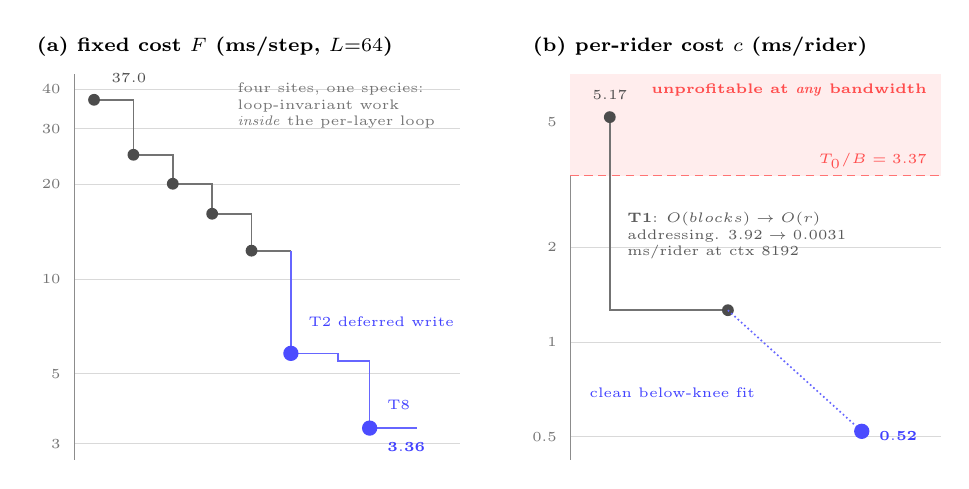
\begin{tikzpicture}[
  x=1cm, y=1cm, font=\scriptsize,
  grid/.style={draw=black!15, very thin},
  pt/.style={circle, fill=black!70, inner sep=0pt, minimum size=1.5mm},
  ptk/.style={circle, fill=blue!70, draw=blue!70, inner sep=0pt, minimum size=1.8mm},
  stair/.style={draw=black!55, semithick},
  ann/.style={font=\tiny, text=black!65, anchor=west},
  axl/.style={font=\tiny, text=black!55, anchor=east},
  tag/.style={font=\scriptsize\bfseries, anchor=west},
]

%% ============ (a) the fixed cost F ============
\node[tag] at (0,5.35) {(a) fixed cost $F$ (ms/step, $L{=}64$)};
\foreach \v/\y in {40/4.808, 30/4.308, 20/3.604, 10/2.400, 5/1.196, 3/0.308} {
  \draw[grid] (0.6,\y) -- (5.5,\y);
  \node[axl] at (0.55,\y) {\v};
}
\draw[black!45] (0.6,0.1) -- (0.6,5.0);

%% the pre-campaign staircase: loop-invariant work inside the per-layer loop
\draw[stair] (0.85,4.674) -- (1.35,4.674) -- (1.35,3.976) -- (1.85,3.976)
             -- (1.85,3.608) -- (2.35,3.608) -- (2.35,3.227) -- (2.85,3.227)
             -- (2.85,2.758) -- (3.35,2.758);
\node[pt] at (0.85,4.674) {};
\node[pt] at (1.35,3.976) {};
\node[pt] at (1.85,3.608) {};
\node[pt] at (2.35,3.227) {};
\node[pt] at (2.85,2.758) {};

%% the campaign
\draw[stair, blue!60] (3.35,2.758) -- (3.35,1.454) -- (3.95,1.454)
             -- (3.95,1.355) -- (4.35,1.355) -- (4.35,0.505) -- (4.95,0.505);
\node[ptk] at (3.35,1.454) {};
\node[ptk] at (4.35,0.505) {};

\node[ann, text=black!70] at (0.95,4.95) {$37.0$};
\node[ann, text=black!55, align=left] at (2.55,4.60)
     {four sites, one species:\\loop-invariant work\\\emph{inside} the per-layer loop};
\node[ann, text=blue!75] at (3.45,1.85) {T2 deferred write};
\node[ann, text=blue!75] at (4.45,0.80) {T8};
\node[ann, text=blue!75, anchor=west] at (4.45,0.26) {$\mathbf{3.36}$};

%% ============ (b) the per-rider cost c, against the gate ============
\begin{scope}[xshift=6.3cm]
\node[tag] at (0,5.35) {(b) per-rider cost $c$ (ms/rider)};
\foreach \v/\y in {5/4.396, 2/2.804, 1/1.600, 0.5/0.396} {
  \draw[grid] (0.6,\y) -- (5.3,\y);
  \node[axl] at (0.55,\y) {\v};
}
\draw[black!45] (0.6,0.1) -- (0.6,5.0);

%% the profitability gate: c must be below T0/B or no rider count ever helps
\fill[red!7] (0.6,3.711) rectangle (5.3,5.0);
\draw[red!55, densely dashed] (0.6,3.711) -- (5.3,3.711);
\node[ann, text=red!70, anchor=east] at (5.25,4.80)
     {\textbf{unprofitable at \emph{any} bandwidth}};
\node[ann, text=red!70, anchor=east] at (5.25,3.90) {$T_0/B = 3.37$};

\draw[stair] (1.1,4.454) -- (1.1,2.002) -- (2.6,2.002);
\node[pt] at (1.1,4.454) {};
\node[pt] at (2.6,2.002) {};
\draw[stair, blue!60, densely dotted] (2.6,2.002) -- (4.3,0.464);
\node[ptk] at (4.3,0.464) {};

\node[ann, text=black!70, anchor=south] at (1.10,4.56) {$5.17$};
\node[ann, text=black!65, anchor=west, align=left] at (1.2,2.95)
     {\textbf{T1}: $O(\text{blocks})\rightarrow O(r)$\\
      addressing. $3.92\rightarrow0.0031$\\
      ms/rider at ctx $8192$};
\node[ann, text=blue!75, anchor=west] at (0.72,0.95)
     {clean below-knee fit};
\node[ann, text=blue!75, anchor=west] at (4.4,0.40) {$\mathbf{0.52}$};
\end{scope}

\end{tikzpicture}}
\caption{\textbf{Both coefficients, as reduced.} In (a) the first four steps are
one species of defect --- loop-invariant work executed inside the per-layer loop;
the worst was a device reduction plus a \texttt{.item()} evaluated once per layer
\emph{inside a guard whose purpose was to skip expensive KV reads}. In (b) the
shaded band is the profitability gate: a host-tier request must cost less than a
resident is worth, $c < T_0/B$, or no rider count helps at any interconnect speed.
The obvious $O(\text{blocks})$ block-table build sits \emph{above} that line, so it
could not have been rescued by a faster link. The dotted segment is a change of
protocol, not a further optimisation --- $5.17$ and $1.26$ were fitted across the
knee, $0.52$ below it --- and the three are therefore not a single ladder.}
\label{fig:ladder}
\end{figure}
